\documentclass{article}

\usepackage{amsmath}
\usepackage{amssymb}
\usepackage{algorithm}
\usepackage[noend]{algpseudocode}		% for algorithms in pseudo code. Usage: \begin{algorithmic}
\MakeRobust{\Call}
\usepackage{tikz}	% for diagrams
\usetikzlibrary{positioning}
\usetikzlibrary{quotes}
% Math mode in tables
\usepackage{array}   % for \newcolumntype macro
\newcolumntype{C}{>{$}c<{$}} % math-mode version of "c" column type

\setlength{\parskip}{\smallskipamount}

\title{Analysis of Algorithms \\
\medskip
\large Homework 4 -- Shortest Path Algorithms}
\author{Abraham Murciano}

\begin{document}

\maketitle

\section{Dijkstra's Algorithm with negative weights}

\subsection*{Part A}

Figure \ref{q1a} shows a graph with negative weights such that if we apply Dijkstra's algorithm to find the shortest path between vertices \(S\) and \(D\), it will return the wrong path.

\begin{figure}[h]
	\centering
	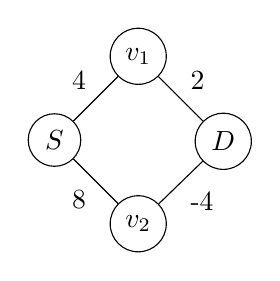
\begin{tikzpicture}
		[vertex/.style={circle, draw=black, node distance=0.8cm}]
		\node[vertex] (S) {\(S\)};
		\node[vertex, above right=of S] (v1) {\(v_1\)};
		\node[vertex, below right=of S] (v2) {\(v_2\)};
		\node[vertex, below right=of v1] (D) {\(D\)};
		\draw (S) to["4"] (v1);
		\draw (S) to["8" below left] (v2);
		\draw (v1) to["2"] (D);
		\draw (v2) to["-4" below right] (D);
	\end{tikzpicture}
	\caption{Graph for which Dijkstra doesn't work}
	\label{q1a}
\end{figure}

Starting off, we assign the unvisited vertices \(v_1\) and \(v_2\) with the distances 4 and 8 respectively, marking \(S\) as visited. Then we take the unvisited vertex with the smallest distance, \(v_1\), and check its neighbours, namely \(D\). We assign it the distance 6 and mark \(v_1\) as visited. Now that our destination vertex is the unvisited vertex with the shortest distance, the algorithm would claim that it has finished, with the shortest path going through \(v_1\) with a distance of 6.

However, in reality the shortest path goes through \(v_2\) and has a total distance of \(8 - 4 = 4\). This path was not considered by the algorithm because the path to the intermediate vertex \(v_2\) has a larger distance than the path it found first.

\subsection*{Part B}

If we take the example graph in figure \ref{q1a} and modify it so that the edges are directed (away from \(S\) or towards \(D\)), then that would form a directed acyclic graph for which Dijkstra's algorithm would not work for a similar reason to that of part A.

\section{Floyd-Warshall with Negative Cycles}

We are to add pseudocode to the Floyd-Warshall algorithm which checks for negative cycles. First, let us take a look at the algorithm.

\begin{algorithm}
	\begin{algorithmic}
		\Function{FloydWarshall}{$V$, $E$}
		\For{\((u,v) \in V \times V\)} \Comment{Initialise all distances to infinity}
		\State \(D_{u,v} := \infty\)
		\EndFor
		\For{\((u,v) \in E\)} \Comment{Apply distances of each edge}
		\State \(D_{u,v} := \Call{Weight}{u, v}\)
		\EndFor
		\For{\(v \in V\)} \Comment{Set distance to itself to zero}
		\State \(D_{v,v} := 0\)
		\EndFor
		\For{\(k \in V\)} \Comment{\(k\) is a possible intermediate vertex between all \((u, v)\)}
		\For{\(u \in V\)}
		\For{\(v \in V\)}
		\State \(D_{u,v} := \Call{Min}{D_{u,k} + D_{k,v}, D_{u,v}}\) \Comment{Seek shorter path via \(k\)}
		\EndFor
		\EndFor
		\EndFor
		\State \Return \(D\)
		\EndFunction
	\end{algorithmic}
\end{algorithm}

Suppose there exists at least one negative cycle (one such that the weights of its edges sum up to a negative number) in a graph \(G = (V, E)\). Now suppose \(a, b \in V\) are two distinct vertices within one such cycle. At the start of the algorithm, \(D_{a,a} = 0\). At some later point in the algorithm, the variables \(u\) and \(v\) will be referring to \(a\) and the variable \(k\) will be referring to \(b\). When this occurs, \(D_{a,a} = 0\) will be compared to \(D_{a,b} + D_{b,a}\). However, we can be certain that \(D_{a,b} + D_{b,a} < 0\), because a path \((a, \dots, b, \dots, a)\) forms a negative cycle. And thus \(D_{a,a}\) will be assigned a negative value.

Therefore, if \(G\) contains negative cycles, when the algorithm concludes, it will tell us that \(\exists v \in V\) such that \(D_{v,v} < 0\). So in order to check if there are negative cycles, we can extend the algorithm as follows.

\begin{algorithm}
	\begin{algorithmic}
		\Function{FloydWarshallNegativeCycles}{$V$, $E$}
		\State \(D := \Call{FloydWarshall}{V, E}\)
		\For{\(v \in V\)}
		\If{\(D_{v,v} < 0\)}
		\State Error: Input contains a negative cycle
		\EndIf
		\EndFor
		\State \Return D
		\EndFunction
	\end{algorithmic}
\end{algorithm}

\section{Shortest Path of Alternating Colour}

We are given a directed, positively weighted graph whose vertices are each either red or blue. We are to write an algorithm which seeks the shortest path from two given vertices, \(v_1\) and \(v_2\), which alternates colours. Meaning if a vertex in the returned path is of one colour, the vertices immediately before and after it must be of the other colour.

This can easily be achieved by removing all edges between two vertices of the same colour, then finding the shortest path with any other algorithm suitable for that purpose.

\begin{algorithm}
	\begin{algorithmic}
		\Function{ShortestAlternatingPath}{$V$, $E$}
		\State \(E' := \phi\)
		\For{\((u, v) \in E\)}
		\If{\(\Call{Colour}{u} \neq \Call{Colour}{v}\)}
		\State insert \((u, v)\) into \(E'\)
		\EndIf
		\EndFor
		\State \Return \Call{ShortestPath}{$V$, $E'$}
		\EndFunction
	\end{algorithmic}
\end{algorithm}

Suppose the complexity of \textsc{ShortestPath} is \(O(f(V, E))\), therefore the complexity of \textsc{ShortestAlternatingPath} would be \(O(E + f(V, E))\), which would change depending on which algorithm was used by \textsc{ShortestPath}.

\section{Running Dijkstra}

We are given the graph in figure \ref{q4}, and told to run Dijkstra's algorithm on it, starting from vertex 2. Table \ref{q4-steps} shows the intermediate values of \(d\) and \(\pi\) throughout the running of the algorithm. Figure \ref{q4-tree} shows the tree of shortest paths returned by the algorithm.

\begin{figure}[htbp]
	\centering
	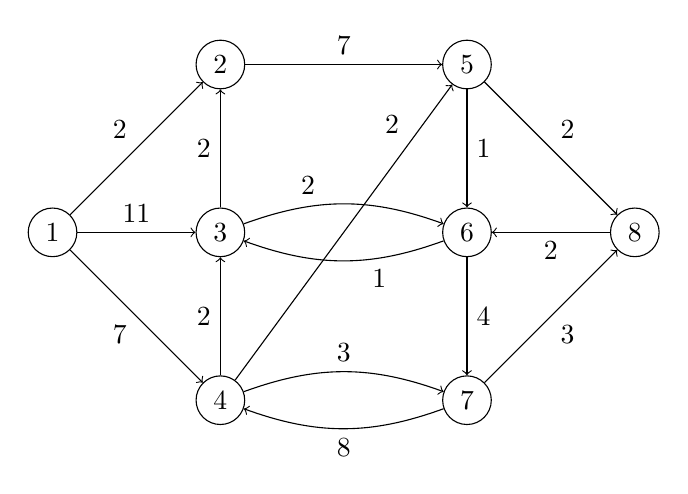
\begin{tikzpicture}
		[vertex/.style={circle, draw=black, node distance=1.5cm}]
		\node[vertex] (1) {1};
		\node[vertex, right=of 1] (3) {3};
		\node[vertex, above=of 3] (2) {2};
		\node[vertex, below=of 3] (4) {4};
		\node[vertex, right=2.5cm of 2] (5) {5};
		\node[vertex, below=of 5] (6) {6};
		\node[vertex, below=of 6] (7) {7};
		\node[vertex, right=of 6] (8) {8};

		\draw[->] (1) to["2"] (2);
		\draw[->] (1) to["11"] (3);
		\draw[->] (1) to["7" below left] (4);
		\draw[->] (3) to["2"] (2);
		\draw[->] (4) to["2"] (3);
		\draw[->] (2) to["7"] (5);
		\draw[->] (4) to["2", pos=0.8] (5);
		\draw[->, bend left=20] (3) to["2", pos=0.4] (6);
		\draw[->, bend left=20] (6) to["1", pos=0.4] (3);
		\draw[->, bend left=20] (4) to["3"] (7);
		\draw[->, bend left=20] (7) to["8"] (4);
		\draw[->] (5) to["1"] (6);
		\draw[->] (6) to["4"] (7);
		\draw[->] (5) to["2"] (8);
		\draw[->] (8) to["2"] (6);
		\draw[->] (7) to["3" below right] (8);
	\end{tikzpicture}
	\caption{A directed positively weighted graph to run Dijkstra on}
	\label{q4}
\end{figure}

\begin{table}[htbp]
	\centering
	\begin{tabular}{||C||C|C||C|C||C|C||C|C||C|C||}
		\hline
		  & d      & \pi & d      & \pi & d      & \pi & d      & \pi & d      & \pi \\
		\hline
		\hline
		1 & \infty & --  & \infty & --  & \infty & --  & \infty & --  & \infty & -- \\
		2 & 0      & --  & 0      & --  & 0      & --  & 0      & --  & 0      & -- \\
		3 & \infty & --  & \infty & --  & \infty & --  & 9      & 6   & 9      & 6 \\
		4 & \infty & --  & \infty & --  & \infty & --  & \infty & --  & 20     & 7 \\
		5 & \infty & --  & 7      & 2   & 7      & 2   & 7      & 2   & 7      & 2 \\
		6 & \infty & --  & \infty & --  & 8      & 5   & 8      & 5   & 8      & 5 \\
		7 & \infty & --  & \infty & --  & \infty & --  & 12     & 6   & 12     & 6 \\
		8 & \infty & --  & \infty & --  & 9      & 5   & 9      & 5   & 9      & 5 \\
		\hline
	\end{tabular}
	\caption{Intermediate values of \(d\) and \(\pi\) for running Dijkstra on the graph in figure \ref{q4}}
	\label{q4-steps}
\end{table}

\begin{figure}[htbp]
	\centering
	\begin{tikzpicture}
		[vertex/.style={circle, draw=black, node distance=1.5cm}]
		\node[vertex] (1) {1};
		\node[vertex, right=of 1] (3) {3};
		\node[vertex, above=of 3] (2) {2};
		\node[vertex, below=of 3] (4) {4};
		\node[vertex, right=2.5cm of 2] (5) {5};
		\node[vertex, below=of 5] (6) {6};
		\node[vertex, below=of 6] (7) {7};
		\node[vertex, right=of 6] (8) {8};
		\draw[->] (6) to["4"] (7);

		\draw[->] (6) to["1" above] (3);
		\draw[->] (7) to["8" above] (4);
		\draw[->] (2) to["7"] (5);
		\draw[->] (5) to["1"] (6);
		\draw[->] (5) to["2"] (8);
	\end{tikzpicture}
	\caption{Tree of shortest paths of the graph in figure \ref{q4} as returned by Dijkstra}
	\label{q4-tree}
\end{figure}

\section{Does a Shortest Path Exist?}

We are given a weighted directed graph \(G\). It is known that there are negative cycles in G. Below is an algorithm that receives source and target vertices, \(s, t \in G\), and checks if a shortest path from \(s\) to \(t\) exists (i.e. there is no negative cycle that can be included in this path).

\begin{algorithm}
	\begin{algorithmic}
		\Function{ExistsShortestPath}{$V, E, s, t$}
		\State \(D := \Call{FloydWarshall}{V, E}\)
		\For{\(v \in V\)}
		\If{\(D_{s,v} + D_{v,t} < \infty\)} \Comment{There is a path from \(s\) to \(t\) via \(v\)}
		\If{\(D_{v,v} < 0\)} \Comment{\(v\) is part of a negative cycle (see question 2)}
		\State \Return false
		\EndIf
		\EndIf
		\EndFor
		\State \Return \(D_{s,t} < \infty\) \Comment{If no path from \(s\) to \(t\) then no shortest path}
		\EndFunction
	\end{algorithmic}
\end{algorithm}

\section{True or False}

For each of these propositions we are to determine whether or not they are true.

\paragraph{Proposition A.} If during the run of Bellman-Ford algorithm for \(i < |V| - 1\) there are no changes applying relaxation, then shortest paths have been found and the run can be halted.

\paragraph{True.} If there are no relaxations in one of the iterations for \(i < |V| - 1\), then nothing will change between iteration \(i\) and iteration \(i+1\). Therefore there will not be any relaxations in iteration \(i+1\). For the same reason there will be no more relaxations for all iterations after the \(i\)\textsuperscript{th}.

\paragraph{Proposition B.} If there is a negative cycle in a graph, then no shortest path between any two vertices can be defined.

\paragraph{False.} There may still be a shortest path between two nodes if there does not exist any path between said nodes which contains any node in the negative cycle.

\section{Bellman-Ford Example}

Figure \ref{q7-graph} shows a graph to run Bellman ford on, starting from vertex \(A\). Table \ref{q7-steps} shows the intermediate values of \(d\) and \(\pi\) throughout the running of the algorithm. Figure \ref{q7-tree} shows the tree of shortest paths returned by the algorithm.

\begin{figure}[htbp]
	\centering
	\begin{tikzpicture}
		[vertex/.style={circle, draw=black, node distance=1.5cm}]
		\node[vertex] (A) {A};
		\node[vertex, right=of A] (C) {C};
		\node[vertex, above=of C] (B) {B};
		\node[vertex, below=of C] (D) {D};
		\node[vertex, right=2.5cm of 2] (E) {E};
		\node[vertex, below=of E] (F) {F};
		\node[vertex, below=of F] (G) {G};
		\node[vertex, right=of F] (H) {H};

		\draw[->] (A) to["2"] (B);
		\draw[->] (A) to["11"] (C);
		\draw[->] (A) to["6" below left] (D);
		\draw[->] (B) to["7"] (E);
		\draw[->] (C) to["2"] (B);
		\draw[->] (C) to["2", pos=0.3] (F);
		\draw[->] (D) to["-2", pos=0.7] (E);
		\draw[->, bend left=20] (D) to["-6"] (G);
		\draw[->] (E) to["-1"] (F);
		\draw[->] (E) to["-2"] (H);
		\draw[->] (F) to["-1"] (G);
		\draw[->, bend left=20] (G) to["9"] (D);
		\draw[->] (G) to["-3" below right] (H);
		\draw[->] (H) to["5"] (F);
	\end{tikzpicture}
	\caption{A directed weighted graph to run Bellman-Ford on}
	\label{q7-graph}
\end{figure}

\begin{table}[htbp]
	\centering
	\begin{tabular}{||C||C|C||C|C||}
		\hline
		  & d      & \pi & d  & \pi \\
		\hline
		\hline
		A & 0      & --  & 0  & -- \\
		B & \infty & --  & 2  & A \\
		C & \infty & --  & 11 & A \\
		D & \infty & --  & 6  & A \\
		E & \infty & --  & 4  & D \\
		F & \infty & --  & 2  & H \\
		G & \infty & --  & 0  & D \\
		H & \infty & --  & -3 & G \\
		\hline
	\end{tabular}
	\caption{Intermediate values of \(d\) and \(\pi\) for running Bellman-Ford on the graph in figure \ref{q7-graph}}
	\label{q7-steps}
\end{table}


\begin{figure}[htbp]
	\centering
	\begin{tikzpicture}
		[vertex/.style={circle, draw=black, node distance=1.5cm}]
		\node[vertex] (A) {A};
		\node[vertex, right=of A] (C) {C};
		\node[vertex, above=of C] (B) {B};
		\node[vertex, below=of C] (D) {D};
		\node[vertex, right=2.5cm of 2] (E) {E};
		\node[vertex, below=of E] (F) {F};
		\node[vertex, below=of F] (G) {G};
		\node[vertex, right=of F] (H) {H};

		\draw[->] (A) to["2"] (B);
		\draw[->] (A) to["11"] (C);
		\draw[->] (A) to["6"] (D);
		\draw[->] (D) to["-2", pos=0.7] (E);
		\draw[->] (D) to["-6"] (G);
		\draw[->] (G) to["-3" below right] (H);
		\draw[->] (H) to["5"] (F);
	\end{tikzpicture}
	\caption{A tree of shortest paths returned by Bellman-Ford from the graph in figure \ref{q7-graph}}
	\label{q7-tree}
\end{figure}

\end{document}